\documentclass{natureprintstyle}
%\documentclass[12pt]{nature}

\spacing{1}
\spacing{2}
\spacing{1}

%\usepackage{epsfig,caption}
\usepackage{amsmath,amssymb}
\usepackage[applemac]{inputenc}
\usepackage{graphicx}
\usepackage{color}
\usepackage{bm}
\usepackage{longtable}
\usepackage{amssymb}
\usepackage{rotating}
\usepackage{hyperref}
%\captionsetup[figure]{labelformat=empty}
%\captionsetup[table]{labelformat=empty}

\newcommand{\gt}{$>$}
\newcommand{\diamonds}{\textsc{D\large{iamonds}}}
\usepackage{hyperref}

\let\citep\cite
\let\citet\cite


\bibliographystyle{naturemag}

\title{\sffamily Dynamical dark energy constraints via clustering shells of SDSS-III BOSS galaxies}

\author{\sffamily 
Xiao-Dong Li,$^{1,\dagger}$
Cristiano G. Sabiu,$^{2}$
Changbom Park,$^{1}$
Yuting Wang,$^{3,\star}$
Gong-bo Zhao,$^{3}$
Hyunbae Park,$^{2}$
Arman Shafieloo,$^{2}$
Juhan Kim,$^{4,1}$
and Sungwook E. Hong$^{2}$}
%Enrico Corsaro$^{1,2,3,4}$, Yueh-Ning Lee$^1$, Rafael A. Garc\'{i}a$^{1}$, Patrick Hennebelle$^1$, Savita Mathur$^{5}$, Paul G. Beck$^1$, Stephane Mathis$^1$, Dennis Stello$^{6,7}$ \& J\'er\^{o}me Bouvier$^8$}

\begin{document}
\maketitle
\let\thefootnote\relax\footnote{


\begin{affiliations}
  \item School of Physics, Korea Institute for Advanced Study, 85 Heogi-ro, Dongdaemun-gu, Seoul 130-722, Korea
  \item Korea Astronomy and Space Science Institute, 776, Daedeokdae-ro, Yuseong-gu, Daejeon, 305-348, Korea
  \item National Astronomy Observatories, Chinese Academy of Science, Beijing, 100012, P.R.China
  \item Center for Advanced Computation, Korea Institute for Advanced Study, 85 Hoegi-ro, Dongdaemun-gu, Seoul 130-722, Korea
\end{affiliations}
}

\vspace{-3.5mm}
\begin{abstract}
\sffamily
We use the anisotropic {\it clustering shells} of 1,133,326 galaxies from the Sloan Digital Sky Survey Data Release 
12 spanning the redshift range $0.15<z<0.69$ to place constraints on the expansion history of the Universe. 
Concentrating on the Chevallier-Polarski-Linder parametrization of dark energy $w=w_0+w_a\frac{z}{1+z}$,
while improving upon earlier works \citep{Li2016}, 
we present a novel use of the Alcock-Paczynski (AP) test via the small scales clustering difference between redshift bins. 
This differential measure appears to be a robust statistical tool which mitigates many systematic effects, 
allowing for competitive and unbiased constrains. 
A combination of CMB+BAO+SNIa+$H_0$+AP yields
$\Omega_m = 0.301 \pm 0.008,\ w_0 = -1.042 \pm 0.067,\ w_a = -0.07 \pm 0.29$ (68.3\% CL).
Adding the AP method reduces the $w_0-w_a$ contour area by 50\%.
The method can be combined with the standard BAO method, 
increasing the science output of ongoing and future galaxy surveys by a factor of 2.
\end{abstract}

\sffamily
{\it Introduction.}---
The  origin  of  the  accelerating  expansion  of  the  universe  is  one of  the  most  salient  questions  in  contemporary cosmology. 
Proposed mechanisms include  evolving  scalar  fields  remnant  from  the  big  bang, 
modifications to gravity,  and a  non-zero  vacuum energy \cite[see][for a comprehensive review]{2012IJMPD..2130002Y}. 
Considering the wealth of theoretical explanations, it is crucial to obtain precise and unbiased measurements of the expansion history of the Universe allowing us to 
differentiate between competing dark energy models.

In recent years the Alcock-Paczynski (AP) test \citep{AP1979} applied to galaxy redshift samples \citep{Outram2004,Blake2011,Alam2016}, 
has allowed tight constraints to be placed on the background averaged distance scales, $D_A(z)$ and $H^{-1}(z)$.  
Assuming an incorrect cosmological model for the coordinate transformation between redshift space and comoving space, produces residual geometric distortions in the resultant galaxy distribution. 
These distortions are induced by the fact that measured distances along 
and perpendicular to the line of sight are fundamentally different. 
Measuring the ratio of galaxy clustering in the radial and transverse directions provides a probe of this AP effect.

%The BAO standard ruler method for obtaining estimates of $D_A(z)$ and $H^{-1}(z)$ is widely used and accepted by the community.
%However, since these measurements are made on large scales (~$120$Mpc), 
%they require large comoving volumes and wide redshift bins to reduce cosmic variance. 
%This results in estimates of the cosmic observables at fewer redshifts and with access to fewer Fourier modes. 
%This reduction of information hinders our attempts to test dark energy models. 

The main caveat of the AP test is due to the fact that 
the radial distances of galaxies are inferred from observed redshifts.
Thus AP tests are inevitably affected by peculiar motions of galaxies,
which leads to apparent anisotropy in the clustering signal, even if the adopted cosmology is correct.
The effect, known as redshift-space distortions (RSD),
is notoriously difficult to model accurately in the 2-point statistics of galaxy clustering \citep{Ballinger1996}.

As alternative methods, \cite{Marinoni2010} proposed using the symmetry properties of galaxy pairs;
however, since the peculiar velocity distorts the redshifts and changes the apparent tilt angles of galaxy pairs,
this method is also seriously limited by RSD \citep{Jennings2011}.
\cite{Ryden1995} and \cite{LavausWandelt1995} proposed another method using the apparent stretching of voids.
This approach has the advantage that the void regions are easier to model compared with dense regions,
but has limitations in that it utilizes only low density regions of the LSS and requires large samples to achieve competitive constraints \citep{Qingqing2016}.

%In an effort to overcome the RSD problem, 
%\citep{Li2016} proposed to apply the AP effect to clustering on small scales. 
%However, redshift space distortions affect the angular clustering of galaxies, mimicking a signal similar to the AP effect, 
%thus contaminating the cosmological information.

In an effort to mitigate the RSD effect, \cite{Li2014} proposed utilizing the {\it redshift dependence} of the AP effect. 
The clustering anisotropies produced by are, although large, close to uniform in magnitude over a wide range in redshift. 
However, if cosmological parameters are incorrectly chosen resulting in an AP effect, 
the anisotropy in the clustering signal has a clear redshift dependence. 
In a later work, \cite{Li2015} developed an AP methodology 
that utilises the redshift dependence of the galaxy 2-point correlation function (2pCF), 
measured as a function of angle between the galaxy pair and line-of-sight (LoS).
As an illustration, Fig.\ref{fig_xy} shows how the shape distortion of objects (anisotropy of clustering signal) varies with distance (or redshift) when incorrect values of  $w_0$ or $w_a$ are used to infer distances.

\citep{Li2016} applied their AP method to galaxies from the 3rd incarnation of the Sloan Digital Sky Survey (SDSS-III).
Combining their method with measurements of the Cosmic Microwave Background (CMB), type Ia supernovae (SNIa), 
baryon acoustic oscillations (BAO), and $H_0$,
they obtained very tight constraints of $ \Omega_m = 0.301 \pm 0.006,\ w=-1.054 \pm 0.025$.
In reducing the RSD effect, 
they were able to use galaxy clustering on scales down to 6 $h^{-1}$Mpc,
which is a major advance in extracting cosmological information 
on small scales where galaxy clustering is strong and there are many independent structures.

In this paper, we continue to develop our previous methodology and proceed to infer the constraints on dynamical dark energy. 
We will present a slightly improved methodology to that of \citep{Li2016}, 
allowing for faster likelihood estimation and thus the exploration of larger, higher dimensional parameter spaces. 
The methodology we will present here, can be applied to any model of dynamical dark energy, 
or indeed any appropriately chosen parametric or non-parametric decomposition of the cosmic expansion history. 
However, as a first step, in this paper we will focus on the widely used Chevallier-Polarski-Linder (CPL) parametrization
$w(z) = w_0 + w_a \frac{z}{1+z}$.


The Planck team has released the {\texttt {COSMOMC}} \citep{LB2002} outputs of four MCMC ``chains'' in the CPL model, 
using a combination of four datasets:
the full-mission Planck observations of CMB temperature and polarization anisotropies \cite{Planck2015},
the BAO distance priors measured from SDSS DR11 \citep{Anderson2013}, 6dFGS \citep{6dFGS} and SDSS MGS \citep{MGS},
the ``JLA'' SNIa sample \citep{JLA},
and the Hubble Space Telescope measurement of $H_0=70.6\pm3.3$ \cite{Riess2011,E14H0}.
These MCMC chains contain the CMB+BAO+SNIa+$H_0$ likelihood computed for $\sim$37,000 sets of cosmological parameters,
yielding constraints of 
\begin{equation}
 \Omega_m = 0.309 \pm 0.010, w_0 = -0.938 \pm 0.109, w_a = -0.38 \pm 0.41.
\end{equation}
%To include the AP method into the constraints,
We then compute the likelihood of the LOWZ+CMASS AP measurements for each of the parameter combinations provided in the Planck chain. 
To do this, we splited the 1,133,326 galaxies from the SDSS DR12 into six redshift bins,
measured the 2pCF in these redshift bins, 
and use a $\chi^2$ function to assess the redshift dependence.
Systematic effects are estimated via mocks made from Horizon Run 4 simulations \citep{HR4}, and subtracted when computing the $\chi^2$.
After adding the sample log-likelihoods with ours, 
while also multiply the sample weights by our likelihoods, 
we derive the CMB+BAO+SNIa+$H_0$+AP constraints on CPL parameters,
\begin{equation}
%\Omega_m = 0.300 \pm 0.008, w_0 = -1.056 \pm 0.061, w_a = -0.04 \pm 0.27,
    %1  0.2999656E+00  0.7616334E-02  0.2958745E+00  0.3035033E+00  0.2878169E+00  0.3132870E+00   \Omega_m
    %2  0.6904801E+00  0.8675444E-02  0.6808558E+00  0.6993898E+00  0.6722945E+00  0.7052207E+00   h
    %3 -0.1056468E+01  0.6096323E-01 -0.1116874E+01 -0.9965903E+00 -0.1175041E+01 -0.9287388E+00   w
    %4 -0.3808376E-01  0.2716607E+00 -0.3105235E+00  0.2321461E+00 -0.6033103E+00  0.4782076E+00   w_a    
\Omega_m = 0.301 \pm 0.008, w_0 = -1.042 \pm 0.067, w_a = -0.07 \pm 0.29.
%    1  0.3014353E+00  0.7759923E-02  0.2974325E+00  0.3048882E+00  0.2889838E+00  0.3152269E+00   \Omega_m
%    2  0.6887652E+00  0.8760036E-02  0.6797134E+00  0.6978279E+00  0.6703971E+00  0.7044224E+00   h
%    3 -0.1041626E+01  0.6732817E-01 -0.1107730E+01 -0.9768319E+00 -0.1172149E+01 -0.8979017E+00   w
%    4 -0.7173374E-01  0.2860547E+00 -0.3572176E+00  0.2107347E+00 -0.6775045E+00  0.4558817E+00   w_a    
\end{equation}
%$$.
While the central values of parameters do not shift appreciably,
the error bars of $w_0$ and $w_a$ are reduced by 38.4\% and 29.7\%, respectively.% $$-40\%$ by adding our method into the analysis.

The marginalised constraints on $w_0-w_a$ are shown in the left panel of Fig.\ref{fig_con}.
Adding our new AP constraints significantly reduces the allowable parameter space. 
This can also be visualise as allowable bands in $w(z)$ as can be seen in the right panel of Fig.\ref{fig_con}.  

The derived cosmological constraints are fully consistent with a cosmological constant dark energy component having no evolution.
Adding the new AP method to the CMB+BAO+SNIa+$H_0$ constraints reduces the statistical errors by $\sim$30-40\%,
and reduces the 95.4\% CL $w_0-w_a$ contour by 50\%.
This reveals the constraining power of the small scale AP effect for probing the redshift evolution of dark energy.

We performed a thorough test of all the possible variables in our methodology.
Figure \ref{fig_contest} shows that,
the result does not change if change them.
%we adopt $\mu_{\rm max}=0.99\ (0.85)$ to include more (less) regions near the LOS,
%decrease the number of angular bins to $n_{\mu}=15-20$,
%change the range of clustering to $8-30 \rm Mpc/h$,
%change the fiducial cosmology to $\Omega_m=0.26,\ w=-0.6$,
%exclude 1 or 2 high redshift bins,
%or reduce the number of mocks to 1000.
The most striking point to note in our testing is that the 
shift in contour position is very small even when we do not include the systematic correction.
This is reassuring, since we may have worried that {\it cosmological dependence} 
on the systematic correction could influence on our final results. 

In sum, \cite{Li2016} proposed to constrain cosmological parameters via 
the redshift dependence of galaxy anisotropic clustering.
This enables a robust AP test on relatively small scales.
In this paper we improved the methodology and obtained tight constraints on the CPL parametrization of dark energy.
%using 1,133,326 galaxies from the Sloan Digital Sky Survey Data Release 
%12 spanning the redshift range $0.15<z<0.69$ . 
%Adding our constraints to the CMB+SNIa+BAO+$H_0$ combination, the $w_0-w_a$ contour was reduced by $\sim50$\%.
The AP method presented in this work has many advantages over the `traditional' galaxy clustering method.
Since it works with the redshift evolution of the anisotropic clustering signal it significantly reduces the effect of systematics. 
It avoids the great difficulty in accurate modelling of the RSD, non-linear clustering and galaxy bias.
It is applicable on much smaller scales, allowing for the inclusion of more $k$-modes and hence more information. 

The presented method of clustering shells can be applied to many spectroscopic galaxy surveys. 
The method is complimentary to the BAO method and the two methods can be combined together, 
increasing (by roughly twice) the science output of ongoing and future surveys, with little to no additional cost.
We expect it play an important role in helping us unveiling the mystery of dark energy.


\begin{thebibliography}{10}
\expandafter\ifx\csname url\endcsname\relax
  \def\url#1{\texttt{#1}}\fi
\expandafter\ifx\csname urlprefix\endcsname\relax\def\urlprefix{URL }\fi
\providecommand{\bibinfo}[2]{#2}
\providecommand{\eprint}[2][]{\url{#2}}


\bibitem[Ade et al. (2015)]{Planck2015}
Ade, P.A.R., Aghanim, N., \& Arnaud, M., et al. arXiv:1502.01589

\bibitem[Alam et al.(2016)]{Alam2016}
Alam, S., Ata, M., \& Bailey, S., et al. 2016,
submitted to MNRAS (arXiv:1607.03155)

%\bibitem[{{Alam} {et~al}\mbox{.}(2015{\natexlab{a}}){Alam}, {Albareti},
%  {Allende Prieto}, {Anders}, {Anderson}, {Anderton}, {Andrews}, {Armengaud},
%  {Aubourg}, {Bailey}, \& et~al.}]{dr12}
%{Alam} S., Albareti, F.D.,\& Allende Prieto, C., {et~al.}, 2015,  ApJS, 219, 12

\bibitem[Alcock \& Paczynski(1979)]{AP1979}
Alcock, C., \& Paczynski, B. 1979, Nature, 281, 358  

%\bibitem[Anderson et al.(2012)]{2012MNRAS.427.3435A} 
%Anderson, L., Aubourg, E., Bailey, S., et al.\ 2012, MNRAS, 427, 3435

\bibitem[Anderson et al.(2013)]{Anderson2013}
Anderson, L., Aubourg, \'E., \& Bailey, S. et al. 2014, MNRAS, 441, 24  
  
%\bibitem[Bassett et al.(2002)]{Bassett2002}
%Bassett, B.A., Kunz, M., Silk, J., \& Ungarelli, C. 2002, MNRAS, 336, 1217

\bibitem[Ballinger, Peacock \& Heavens 1996]{Ballinger1996}
Ballinger, W.E., Peacock, J.A., \& Heavens, A.F. 1996, MNRAS, 282, 877  

\bibitem[Betoule et al.(2014)]{JLA}
Betoule, M., Kessler, R., \& Guy, J., et al. 2014, A\&A, 568, 32


\bibitem[Beutler et al.(2011)]{6dFGS}
Beutler, F., Blake, C., \& Colless, M., et al. 2011, MNRAS, 416, 3017

\bibitem[Beutler et al.(2013)]{Beutler2013}
Beutler, F., Saito, S., \& Seo, H.-J., et al. 2013, MNRAS, 443, 1065

\bibitem[Beutler et al.(2016)]{Beutler2016}
Beutler, F., Seo, H.-J., \& Saito, S., et al. 2016,
arXiv:1607.03150

\bibitem[Blake et al.(2011)]{Blake2011}
Blake, C., Glazebrook, K., \& Davis, T. M., 2011, MNRAS, 418, 1725  

\bibitem[Blake et al.(2013)]{WiggleZtopoloy}
Blake, C., James, J.B., \& Poole, G.B. 2013, MNRAS, 437, 2488

\bibitem[Bolton et al.(2012)]{Bolton2012}
Bolton, A.S., Schlegel, \& D.J., Aubourg E., et al. 2012, AJ, 144, 144

\bibitem[Boylan-Kolchin et al.(2008)]{B08}
Boylan-Kolchin, M., Ma, C.-P., \& Quataert, E. 2008, MNRAS, 383, 93


%\bibitem[Bueno Belloso et al. (2012)]{BB2012}
%Bueno Belloso, A., Pettinari, G.W., Meures, N., \& Percival, W.J. 2012, Phys. Rev. D, 86, 023530

%\bibitem[Chevallier \& Polarski(2001)]{CP2001}
%Chevallier, M., Polarski, D. 2001, Int. J. Mod. Phys. D, 10, 213


%\bibitem[Choi et al.(2010)]{choi 2010}
%Choi, Y.-Y., Park, C., Kim, J., Gott, J.R., 
%Weinberg, D.H., Vogeley, M.S., \& Kim, S.S. 2010, ApJS, 190, 181

\bibitem[Christensen et al.(2001)]{Bayesian}
Christensen, N., Meyer, R., Knox, L., \& Luey, B. 2001, Class. Quant. Grav., 18, 2677

%\bibitem[Chuang et al.(2013)]{Chuang2013}
%Chuang, C.-H., Prada, F., Beutler, F., et al. 2013, arXiv:1312.4889  

\bibitem[Chuang \& Wang(2012)]{ChuangWang2012}
Chuang, C.-H., \& Wang, Y. 2012, MNRAS, 426, 226  


%\bibitem[Corasaniti \& Copeland(2003)]{Corasaniti2003}
%Corasaniti, P.S., Copeland, E.J. 2003, Phys. Rev. D, 67, 063521

%eBOSS: 
%http://arxiv.org/abs/1508.04473
\bibitem[Dawson et al.(2015)]{eBOSS}
Dawson, K.S., Kneib, J.P., \& Percival, W.J., et al. 2015, accepted AJ

\bibitem[Dawson et al.(2012)]{Dawson et al. 2012}
Dawson, K.S., Schlegel, D.J., \& Ahn, C.P., et al. 2012, AJ, 145, 10

\bibitem[Efstathiou (2014)]{E14H0}
Efstathiou, G. 2014, MNRAS, 440, 1138

\bibitem[Eisenstein et al.(2011)]{Eisenstein et al. 2011}
Eisenstein, D.J.,  Weinberg, D.H., \& Agolet, E., et al. 2011, AJ, 142, 72

\bibitem[Feldman, Kaiser \& Peacock (1994)]{1994ApJ...426...23F} 
Feldman, H.A., Kaiser, N., \& Peacock, J.A.\ 1994, ApJ, 426, 23 

\bibitem[Fukugita et al. (1996)]{Fukugita1996}
Fukugita, M., Ichikawa, T., \& Gunn, J.E., et al. 1996, AJ, 111, 1748
%Publication:	
%Astronomical Journal v.111, p.1748 

%\bibitem[Gingold \& Monaghan(1977)]{GM1977}
%Gingold, R.A., \& Monaghan, J.J. 1977, MNRAS, 181, 375  

%\bibitem[Gott et al.(2009)]{gott 2009}
%Gott, J.R., Choi, Y.-Y., Park, C., \& Kim, J. 2009, ApJ, 695, L45  

%\bibitem[Gott et al.(2008)]{gott 2008}
%Gott, J.R., Hambrick, D.C., Vogeley, M.S., Kim, J., Park, C., Choi, Y.-Y.,
%Cen, R., Ostriker, J.P., \& Nagamine, K. 2008, ApJ, 675, 16  


\bibitem[Gunn et al. (1998)]{Gunn1998}	
Gunn, J.E., Carr, M., \& Rockosi, C. et al. 1998, AJ, 116, 3040

\bibitem[Gunn et al.(2006)]{Gunn et al. 2006}
Gunn, J.E., Siegmund, W.A., \& Mannery, E.J., et al. 2006, AJ, 131, 2332

\bibitem[Guzzo et al.(2008)]{Guzzo2008}
Guzzo, L., Pierleoni, M., \& Meneux, B., et al. 2008, Nature, 451, 541

\bibitem[Hartlap et al.(2006)]{Hartlap}
Hartlap J., Simon P. \& Schneider P. [astro-ph/0608064].


\bibitem[Hong et al.(2016)]{hong2016}
Hong, S.E., Park, C.,\&  Kim, J. 2016, ApJ, 823, 103

\bibitem[Jackson (1972)]{FOG}
Jackson, J., 1972, MNRAS, 156, 1

\bibitem[Jennings et al.(2011)]{Jennings2011}
Jennings, E., Baugh, C.M., \& Pascoli, S. 2011, MNRAS, 420, 1079  

%\bibitem[Jeong et al.(2014)]{Jeong2014}
%Jeong, D., Dai, L., Kamionkowski, M., \& Szalay, A.S. 2014, arXiv:1408.4648

\bibitem[Jiang et al.(2008)]{jiang2008}
Jiang, C.Y., Jing, Y. P., \& Faltenbacher, A., et al. 2008, ApJ, 675, 1095

\bibitem[Kaiser (1987)]{Kaiser1987}
Kaiser, N. 1987, MNRAS, 227, 1


\bibitem[Kim \& Park(2006)]{kim and park 2006}
Kim, J., \& Park, C. 2006, ApJ, 639, 600  

\bibitem[Kim et al.(2009)]{2009ApJ...701.1547K} 
Kim, J., Park, C., Gott, J.R., III, \& Dubinski, J.\ 2009, ApJ, 701, 1547 

\bibitem[Kim et al.(2015)]{hr4}
Kim, J., Park, C., L'Huillier, B., \& Hong, S. E. 2015, JKAS, 48, 213

\bibitem[Kim et al.(2011)]{horizonrun}
Kim, J., Park, C., Rossi, G., Lee, S.M., \& Gott, J.R. 2011, JKAS, 44, 217  

\bibitem[Kitaura et al.(2015)]{MDPATCHY}
Kitaura, F.S., Rodriguez-Torres, S., Chuang, C.-H., et al. arXiv:1509.06400

\bibitem[Komatsu et al.(2011)]{komatsu 2011}
Komatsu, E., Smith, K. M., \& Dunkley, J., et al. 2011, ApJS, 192, 18  

\bibitem[Lacey \& Cole(1993)]{LC93}
Lacey, C., \& Cole, S. 1993, MNRAS, 262, 627


\bibitem[Landy \& Szalay(1993)]{1993ApJ...412...64L} 
Landy, S.D., \& Szalay, A.S.\ 1993, ApJ, 412, 64 

%EUCLID:
%http://arxiv.org/abs/1110.3193
\bibitem[Laureijs et al.(2011)]{EUCLID}
Laureijs, R., Amiaux, J., \& Arduini, S., et al. 2011, arXiv:1110.3193

\bibitem[Lavaux \& Wandelt(2012)]{LavausWandelt1995}
Lavaux, G., \& Wandelt, B.D. 2012, ApJ, 754, 109  

%\bibitem[Levi et al.(2013)]{2013arXiv1308.0847L} 
%Levi, M., Bebek, C., Beers, T., et al.\ 2013, arXiv:1308.0847 

\bibitem[Lewis \& Bridle (2002)]{LB2002}
Lewis, A., \& Bridle, S. 2002, Phys. Rev. D, 66, 103511

\bibitem[L'Huillier et al.(2014)]{2014NewA...30...79L} 
L'Huillier, B., Park, C., \& Kim, J.\ 2014, New Astronomy, 30, 79 

\bibitem[Li et al.(2011)]{Li2011}
Li, M., Li, X.-D., Wang, S., \& Wang, Y. 2011, Commun. Theor. Phys., 56, 525

\bibitem[Li et al.(2014)]{Li2014}
Li, X.-D., Park, C., Forero-Romero, J., \& Kim, J. 2014, ApJ, 796, 137

\bibitem[Li et al.(2015)]{Li2015}
Li, X.-D., Park, C., Sabiu, C.G., \& Kim, J. 2015, MNRAS, 450, 807 

\bibitem[Li et al.(2016)]{Li2016}
Li, X.-D., Park, C., \& Sabiu, C.G., et al. 2016, ApJ, 832, 103

%\bibitem[Linder(2003)]{Linder2003}
%Linder, E.V. 2003, Phys. Rev. Lett., 90, 091301

\bibitem[Linder et al.(2014)]{Linder2013}
Linder, E.V., Minji, O., Okumura, T., Sabiu, C.G., \& Song, Y.-S. 2014, Phys. Rev. D, 89, 063525  

\bibitem[L{\'o}pez-Corredoira(2014)]{2014ApJ...781...96L} 
L{\'o}pez-Corredoira, M.\ 2014, ApJ, 781, 96 

\bibitem[Mao et al. (2016)]{Qingqing2016}
Mao, Q., Berlind, A.A., Scherrer, R.J., et al. 2016, submitted to ApJ

\bibitem[Marinoni \& Buzzi(2010)]{Marinoni2010}
Marinoni, C., \& Buzzi, A. 2010, Nature, 468, 539  

\bibitem[Matsubara \& Suto(1996)]{Matsubara1996}
Matsubara T., \& Suto, Y. 1996, ApJ, 470, L1  

\bibitem[McCavana et al.(2012)]{M12}
McCavana, T., Micic, M., Lewis, G. F., et al. 2012, MNRAS, 424, 361


\bibitem[Morandi \& Sun (2016)]{MS2016}
Morandi, A., \& Sun, M. arXiv:1601.03741


\bibitem[Outram et al.(2004)]{Outram2004}
Outram, P.J., Shanks, T., Boyle, B.J., Croom, S.M., Hoyle, F., Loaring, N.S., 
Miller, L., \& Smith, R.J. 2004, MNRAS, 348, 745  

%\bibitem[Parejko et al.(2013)]{Parejko2013}
%Parejko, J. K., Sunayama, T., Padmanabhan, N., et al. 2013, MNRAS, 429, 98  

\bibitem[Parejko et al.(2013)]{Parejko2013}
Parejko J.K., et al., 2013, MNRAS, 429, 98

\bibitem[Parihar et al. (2014)]{CMASSLSS2014}
Parihar, P., Vogeley, M.S., \& Gott, J.R., et al. 2014, ApJ, 796, 86

\bibitem[Park et al.(2005)]{park 2005}
Park, C., Kim, J., \& Gott, J.R. 2005, ApJ, 633, 1  

\bibitem[Park \& Kim(2010)]{topology}
Park, C., \& Kim, Y.-R. 2010, ApJL, 715, L185  

\bibitem[Park et al. (2012)]{Park2012}
Park, C., Choi, Y.-Y., Kim, J., Gott, J.R., Kim, S.S., \&
Kim, K.-S. 2012, ApJ, 759, 7

\bibitem[Park et al. (2015)]{Park2015}
Park, C., Song, H., Einasto, M., Lietzen, H., \&
Heinamaki, P. 2015, JKAS, 48, 75

\bibitem[Peebles \& Ratra(2003)]{PR2003}
Peebles, P.J.E., \& Ratra, B. 2003, Reviews of Modern Physics, 75, 559

\bibitem[Percival et al.(2014)]{Percival2014}
Percival, W.J., Ross, A.J., \& S\'{a}nchez, A.G., et al. 2014, MNRAS, 439, 2531

\bibitem[Perlmutter et al.(1999)]{Perl1999}
Perlmutter, S., Aldering, G., \& Goldhaber, G., et al. 1999, ApJ, 517, 565  

\bibitem[Press \& Shechter(1974)]{PS1974}
Press, W.H., \& Schechter, P.L. 1974, ApJ, 187, 425



\bibitem[Reid et al.(2012)]{Reid2012}
Reid, B., Samushia, L., \& White, M., et al. 2012, MNRAS, 426, 2719  

\bibitem[Reid et al.(2016)]{Reidetal:2016}
Reid, B., Ho, S., \& Padmanabhan, N., et al.  2016, MNRAS, 455, 1553

\bibitem[Riess et al.(1998)]{Riess1998}
Riess, A.G., Filippenko, A.V., \& Challis, P., et al. 1998, AJ, 116, 1009  

\bibitem[Riess et al.(2011)]{Riess2011}
Riess, A.G., Macri, L., \& Casertano, S., et al. 2011, ApJ, 730, 119
%A 3\% Solution: Determination of the Hubble Constant with the Hubble Space Telescope and Wide Field Camera

\bibitem[Ross et al.(2012)]{2012MNRAS.424..564R} 
Ross, A.J., Percival, W.J., \& S{\'a}nchez, A.G. et al.\ 2012, MNRAS, 424, 564 

\bibitem[Ross et al.(2015)]{MGS}
Ross, A.J., Samushia, L., \& Howlett, C., et al. 2015, MNRAS, 449, 835

\bibitem[Ryden(1995)]{Ryden1995}
Ryden, B.S. 1995, ApJ, 452, 25  

%\bibitem[Samushia et al.(2014)]{Samushia2014}
%Samushia, L., Reid, B. A., White, M., et al. 2014, MNRAS, 439, 3504  

%\bibitem[Sanchez et al.(2013)]{Sanchez2013}
%Sanchez, A. G., Kazin, E. A., Beutler, F., et al. 2013, MNRAS, 433, 1202  

%\bibitem[Sutter et al.(2014)]{Sutter2014}
%Sutter, P.M., Pisani, A., Wandelt, B.D., \& Weinberg, D.H. 2014, MNRAS, 443, 2983

\bibitem[Sanchez et al.(2016)]{Sanchez2016}
Sanchez, A. G., Scoccimarro, R., \& Crocce, M., et al.
arXiv:1607.03147

\bibitem[Schlafly et al.(2010)]{Schlafly2010}
Schlafly E.F., Finkbeiner D.P., Schlegel D.J., et al. 2010, ApJ, 725, 1175

\bibitem[Schlafly \& Finkbeiner(2011)]{SF2011}
Schlafly E.F., \& Finkbeiner D.P. 2011, ApJ, 737, 103


%DESI:
%http://arxiv.org/abs/1106.1706
\bibitem[Schlegel et al.(2011)]{DESI}
Schlegel, D., Abdalla, F., \& Abraham, T., et al. 2011, arXiv:1106.1706

\bibitem[Smee et al.(2013)]{Smee2013}
Smee, S.A., Gunn, J.E., \& Uomoto, A., et al. 2013, AJ, 146, 32

\bibitem[Song et al.(2014)]{2014arXiv1407.2257S} 
Song, Y.S., Sabiu, C.G., 
Okumura, T., Oh, M., \& Linder, E.V.\ 2014, JCAP, 12, 005 

\bibitem[Speare et al. (2015)]{Speare2015}
Speare, R., Gott, J.R., Kim, J., \& Park, C.
2015, ApJ, 799, 176

%\bibitem[Tojeiro \& Percival(2011)]{Tojeiro2011}
%Tojeiro R., \& Percivial W.J. 2011, MNRAS, 417, 1114  

%\bibitem[Tojeiro et al.(2012)]{Tojeiro2012}
%Tojeiro, R., Percival, W. J., Wake, D. A., et al. 2012, MNRAS, 424, 136 

\bibitem[Viana \& Liddle(1996)]{VL1996}
Viana, P.T.P., \& Liddle, A.R. 1996, MNRAS, 281, 323

\bibitem[Villalobos et al.(2013)]{V13}
Villalobos, \'{A}., ́De Lucia, G., Weinmann, S.M., Borgani, S., \& Murante, G. 2013, MNRAS, 433, L49


\bibitem[Weinberg (1989)]{SW1989}
Weinberg, S. 1989, Reviews of Modern Physics, 61, 1

\bibitem[White (2011)]{White2011}
White M., et al. 2011, ApJ, 728, 126

\bibitem[Yoo \& Watanabe(2012)]{2012IJMPD..2130002Y} Yoo, J., \& Watanabe, Y.\ 2012, International Journal of Modern Physics D, 21, 1230002 

\bibitem[York et al.(2000)]{York et al. 2000}
York, D.G., Adelman, J., \& Anderson, J.E., et al. 2000, AJ, 120, 1579

\bibitem[Zehavi et al.(2011)]{zehavi2011}
Zehavi, I., Zheng, Z., \& Weinberg, D.H., et al. 2011, ApJ, 736, 59

%\bibitem{Milliman14}
%\bibinfo{author}{Milliman}, K.~E. {\it et~al.}
%\newblock \bibinfo{title}{WIYN Open Cluster Study. LX. Spectroscopic Binary Orbits in NGC 6819.}
%\newblock{\it Astron. \ J.}{\bf\, 148}, 38--57 (2014).

\end{thebibliography}

\begin{addendum}
\item [Acknowledgements] 
We thank the Korea Institute for Advanced Study for providing computing resources (KIAS Center for Advanced Computation Linux Cluster System).
CGS acknowledges support from the National Research Foundation (NRF,  \#2017R1D1A1B03034900). 
We thank Stephen Appleby, Seokcheon Lee, Maurice van Putten, Graziano Rossi and Yi Wang for helpful discussions.


\item[Author contributions] 

X.L. computed the approximated 2pCFs in the many cosmologies, computed the likelihoods based on them, derived the final cosmological constraints, and did the robustness tests. 
C.S. wrote the code computing the 2pCFs, and contributed in the likelihood analysis and the robustness tests. 
C.P. proposed the concept of using redshift dependence to do AP tests, and have extensive discussions with X.L. about the likelihood analysis, 
systematic correction, and robustness tests.
Y.W. and G.Z. contributed in the computing the approximated 2pCFs in non-fiducial cosmologies, and the robustness tests.
H.P. contributed in the cross-check of the 2pCF measurements, the likelihood analysis, and the systematic correction.
A.S. contributed in the fast likelihood in non-fiducial cosmologies and the cosmological interpretation of the results.
J.K. and S.H. performed the Horizon Run 4 simulations and built the mock galaxy samples.
All authors commented on the manuscript.


\item[Author information]
%Supplementary information is available for this paper. 
Reprints and permissions information is available at \href{www.nature.com/reprints}{www.nature.com/reprints}.
Correspondence and requests for materials should be addressed to X.D. (e-mail: \href{mailto:xiaodongli@kias.re.kr}{xiaodongli@kias.re.kr}).

\item[Competing interests]
The authors declare no competing financial interests.

\end{addendum}



\newpage

\begin{figure}[tb]
   \centering{
   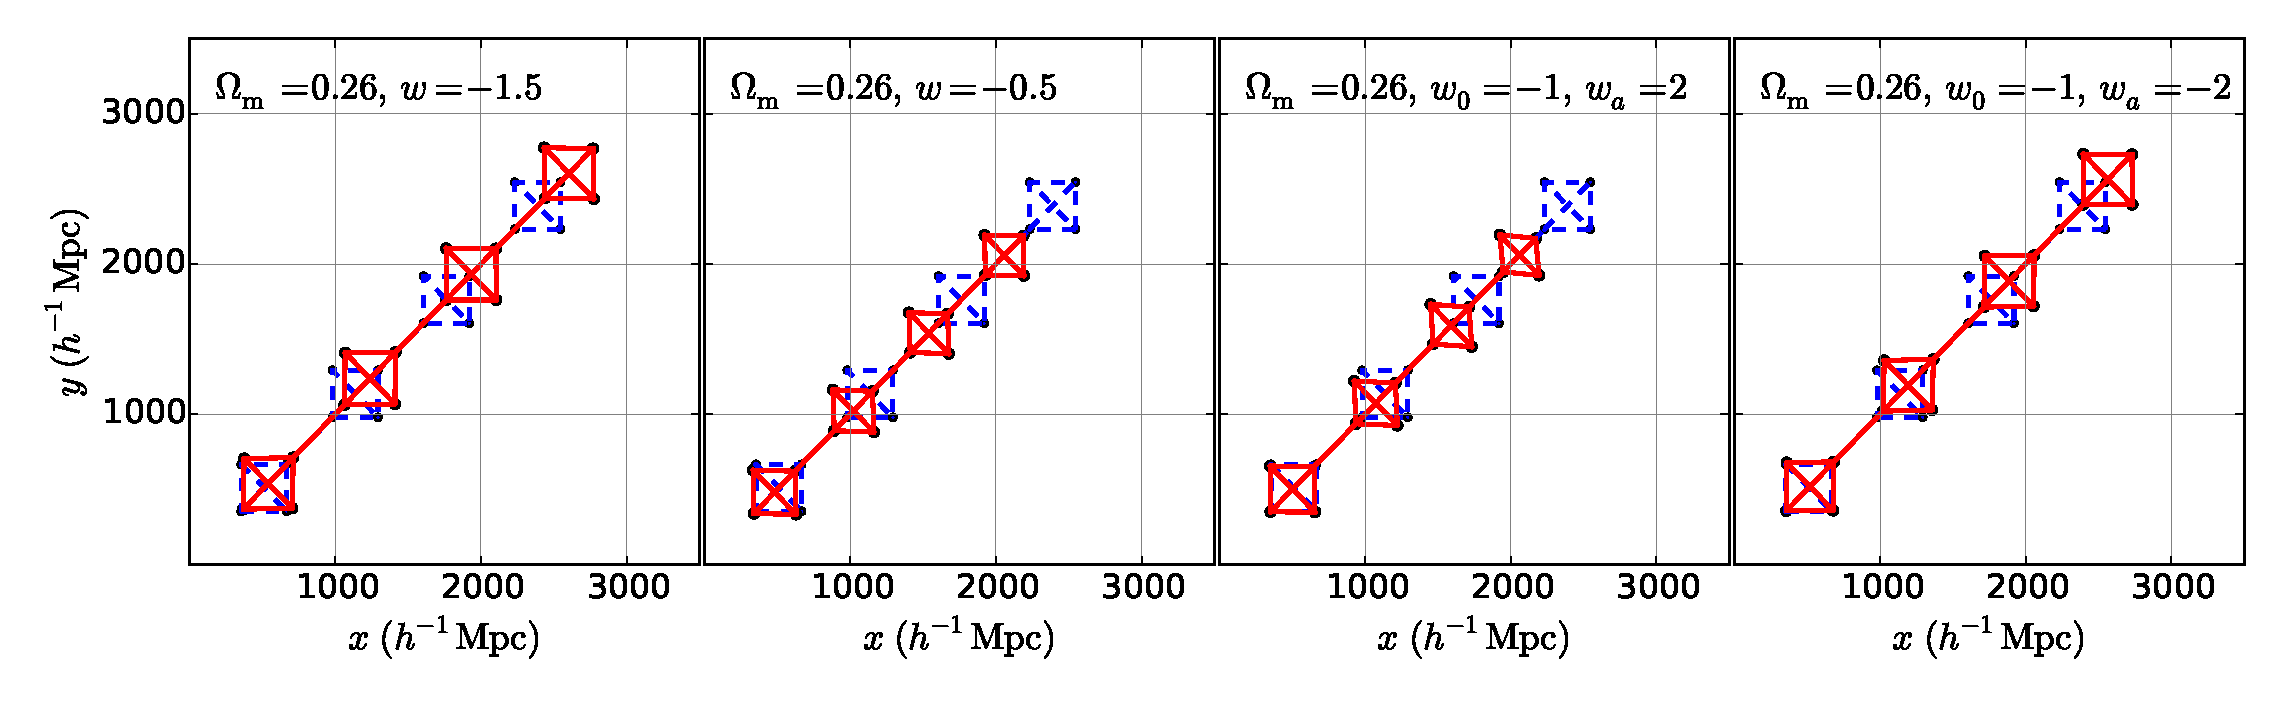
\includegraphics[height=5cm]{fig_xy.eps}
   }
   \vspace{-2mm}
   \caption{\label{fig_xy}
   The distance dependence of the shape distortion in four wrongly assumed cosmologies,
   assuming a true cosmology of $\Omega_m=0.31$, $w=-1$.
   There are four perfect squares with their true shapes plotted in blue dashed lines.
   They are measured by an observer located at the origin, and the distances are reprojected in the four wrong cosmologies.
   The apparently distorted shapes are plotted in red solid lines.
   }
   \vspace{-4mm}
\end{figure}

\begin{figure}[tb]
   \centering{
   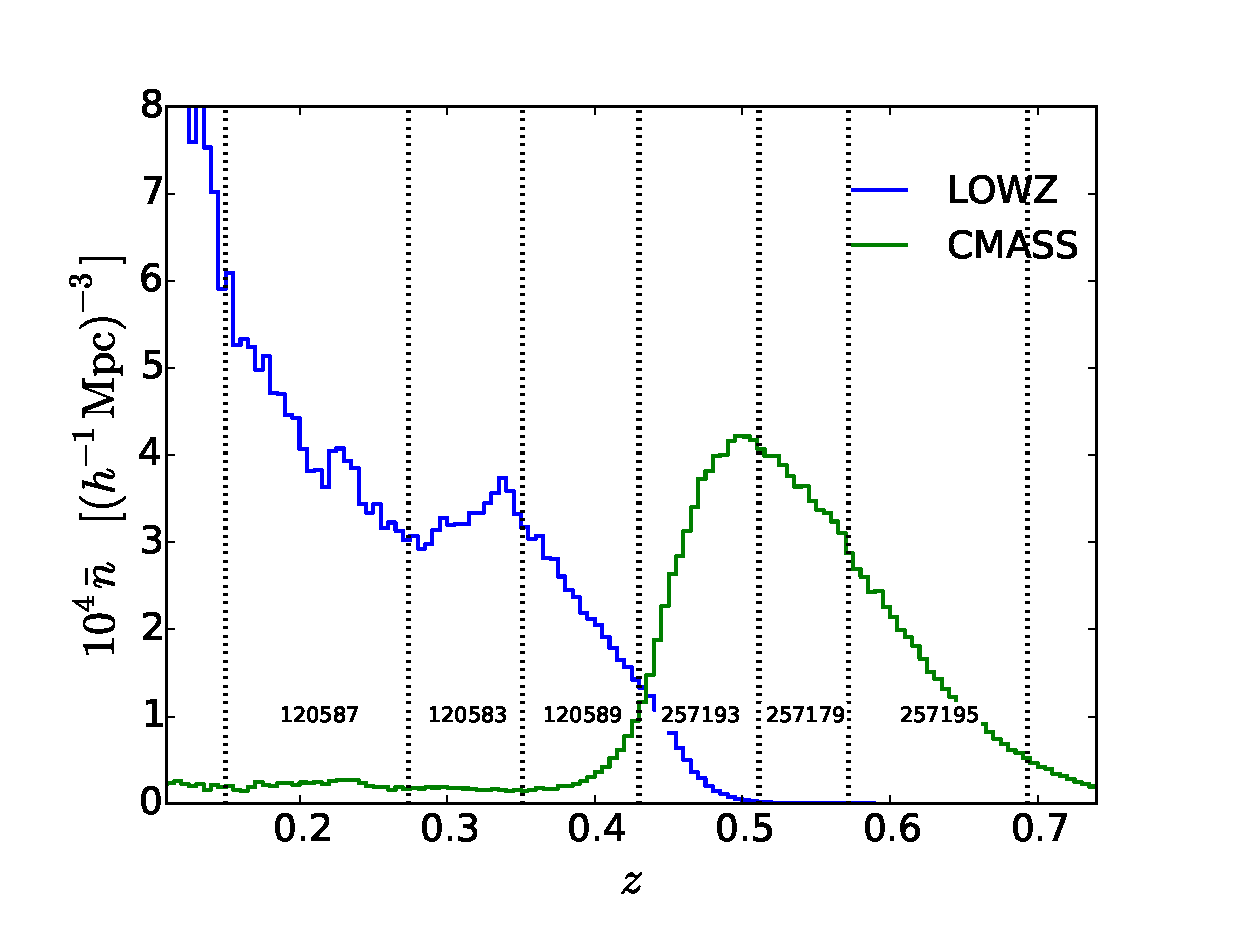
\includegraphics[height=5.3cm]{fig_nbar.eps}
   \includegraphics[width=7cm,]{fig_2pcf.eps}
   }
   \caption{\label{fig_TpCF}
   Left panel: We split the BOSS DR12 galaxies into six redshift bins to measure the evolution of shape distortion.
   The blue and green solid histograms show the redshift density distribution of LOWZ and CMASS galaxies in the $\Omega_m=0.31$ $\Lambda$CDM. 
   The vertical dashed lines define the six redshift bins that are used to cut the samples.                                       .
   The number of LOWZ/CMASS galaxies in the three low/high redshift bins are listed.
   Right panel: 2D contour map of measured $\xi$ as a function of $\mu$ and $s$, from the six redshift bins of LOWZ and CMASS samples, 
      in the cosmology of $\Omega_m=0.31$ $\Lambda$CDM model.
    The black dashed lines mark the clustering region 6-40\ Mpc/h studied in the AP method.
    The six contour maps have rather similar appearance, implying small redshift evolution of $\xi$ from RSD.
   }
\end{figure}

\begin{figure}[tb]
   \centering{
   \includegraphics[height=5cm,natwidth=6,natheight=4.5]{figCPL_b.pdf}
   %\includegraphics[width=5.5cm,natwidth=4,natheight=4]{figCPL_b_BAOSNIaAP.pdf}
   \includegraphics[height=5cm,natwidth=6,natheight=4.5]{figCPL_d.pdf}
   }
   \caption{\label{fig_con}
   Left panel: 68.3\%, 95.4\% CL likelihood contours in the  $w_0-w_a$ plane.
   %Results are consistent with $\Lambda$CDM.
   The constrained area is significantly reduced after combined with the AP method.
   %This shows the power of the AP method in constraining dynamical dark energy.
   %Middle panel: $w_0-w_a$ likelihood contours using datasets of CMB+BAO, CMB+BAO+SNIa+$H_0$ and CMB+BAO+AP+$H_0$.
   %When combined with CMB+BAO, AP method yields much tighter constraints than SNIa.
   Right panel: Redshift evolution of $w(z)$, with/without adding the AP constraint.
   Adding AP tightens the constraints and reduces the redshift evolution of $w$ (tilt of $w(z)$).
   }
\end{figure}

\begin{figure}[tb]
   \centering{
   \includegraphics[width=16cm,natwidth=6,natheight=5]{fig_con_tests.pdf}
   %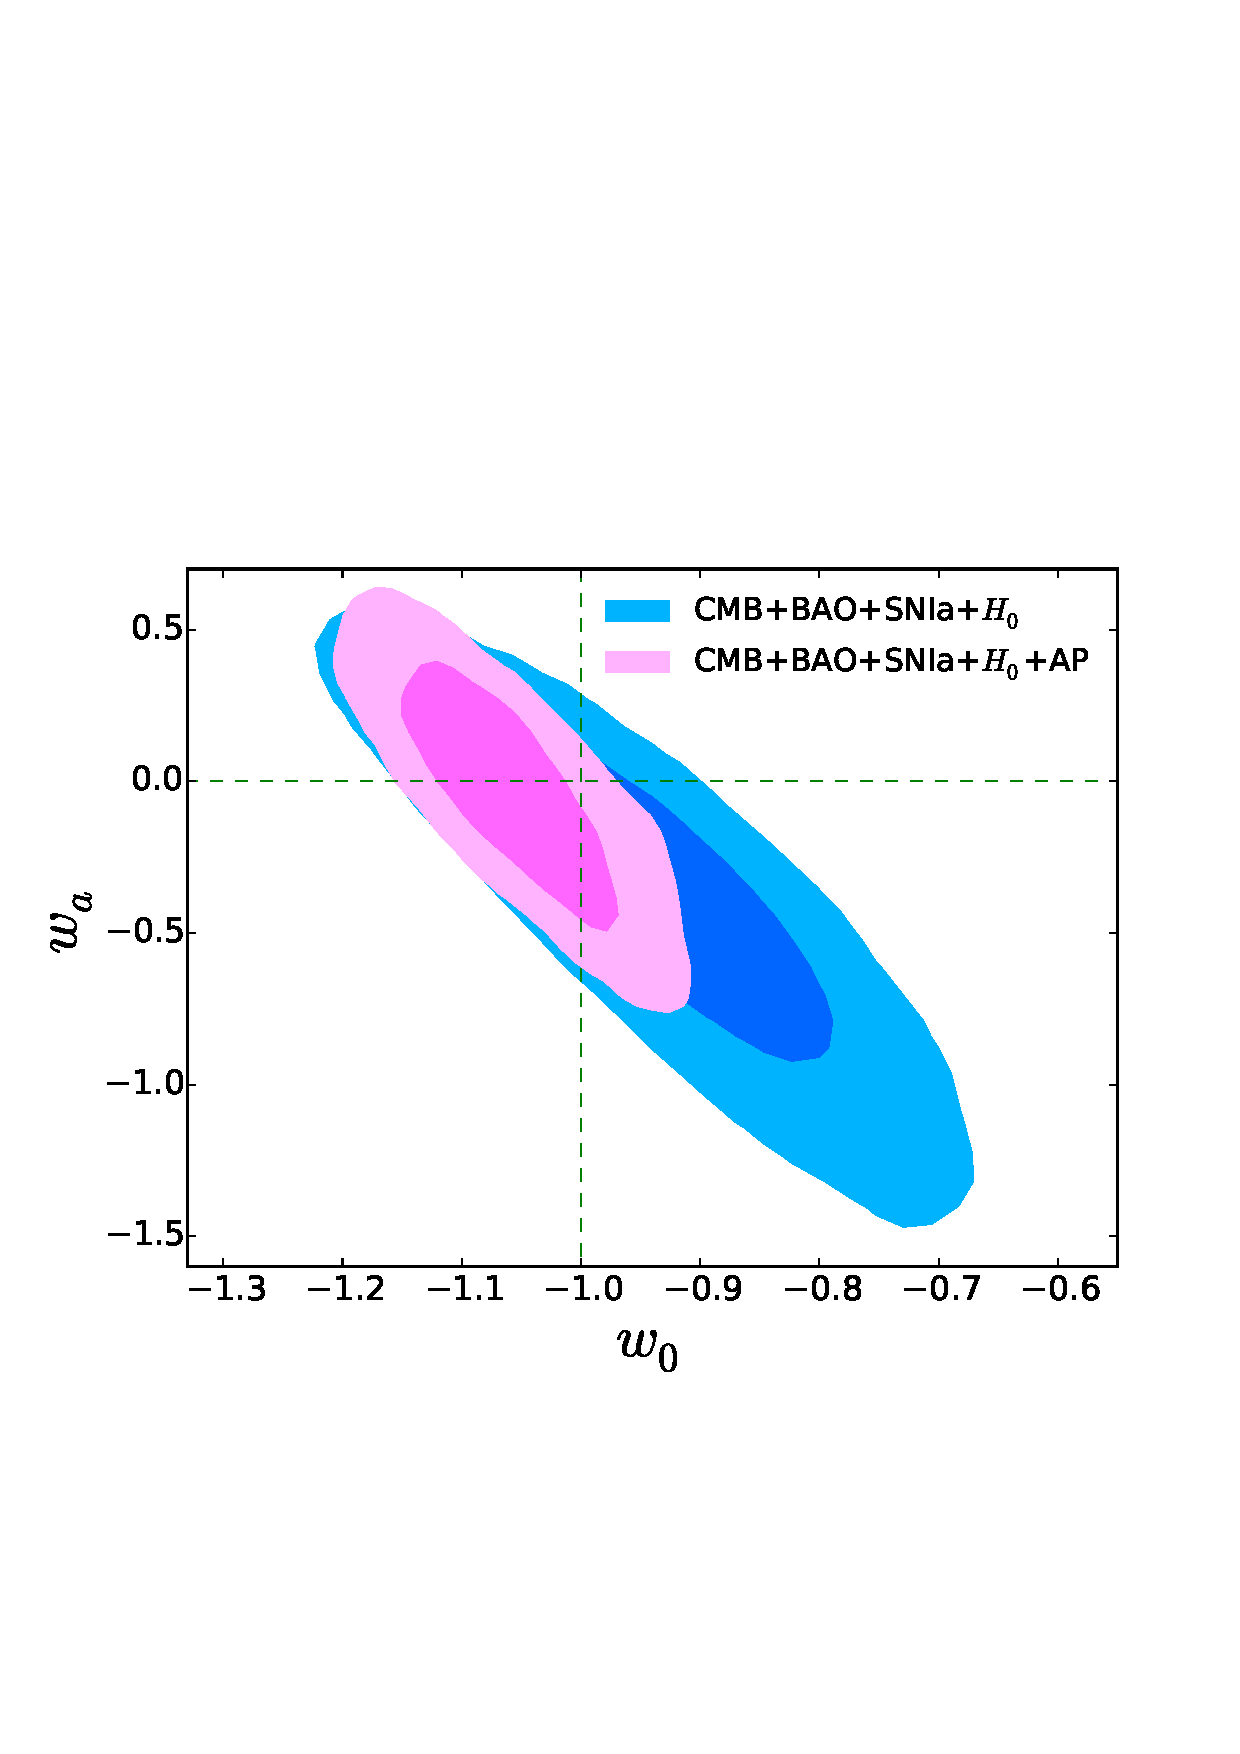
\includegraphics[width=9cm,natwidth=4,natheight=4]{fig2b.pdf}
   %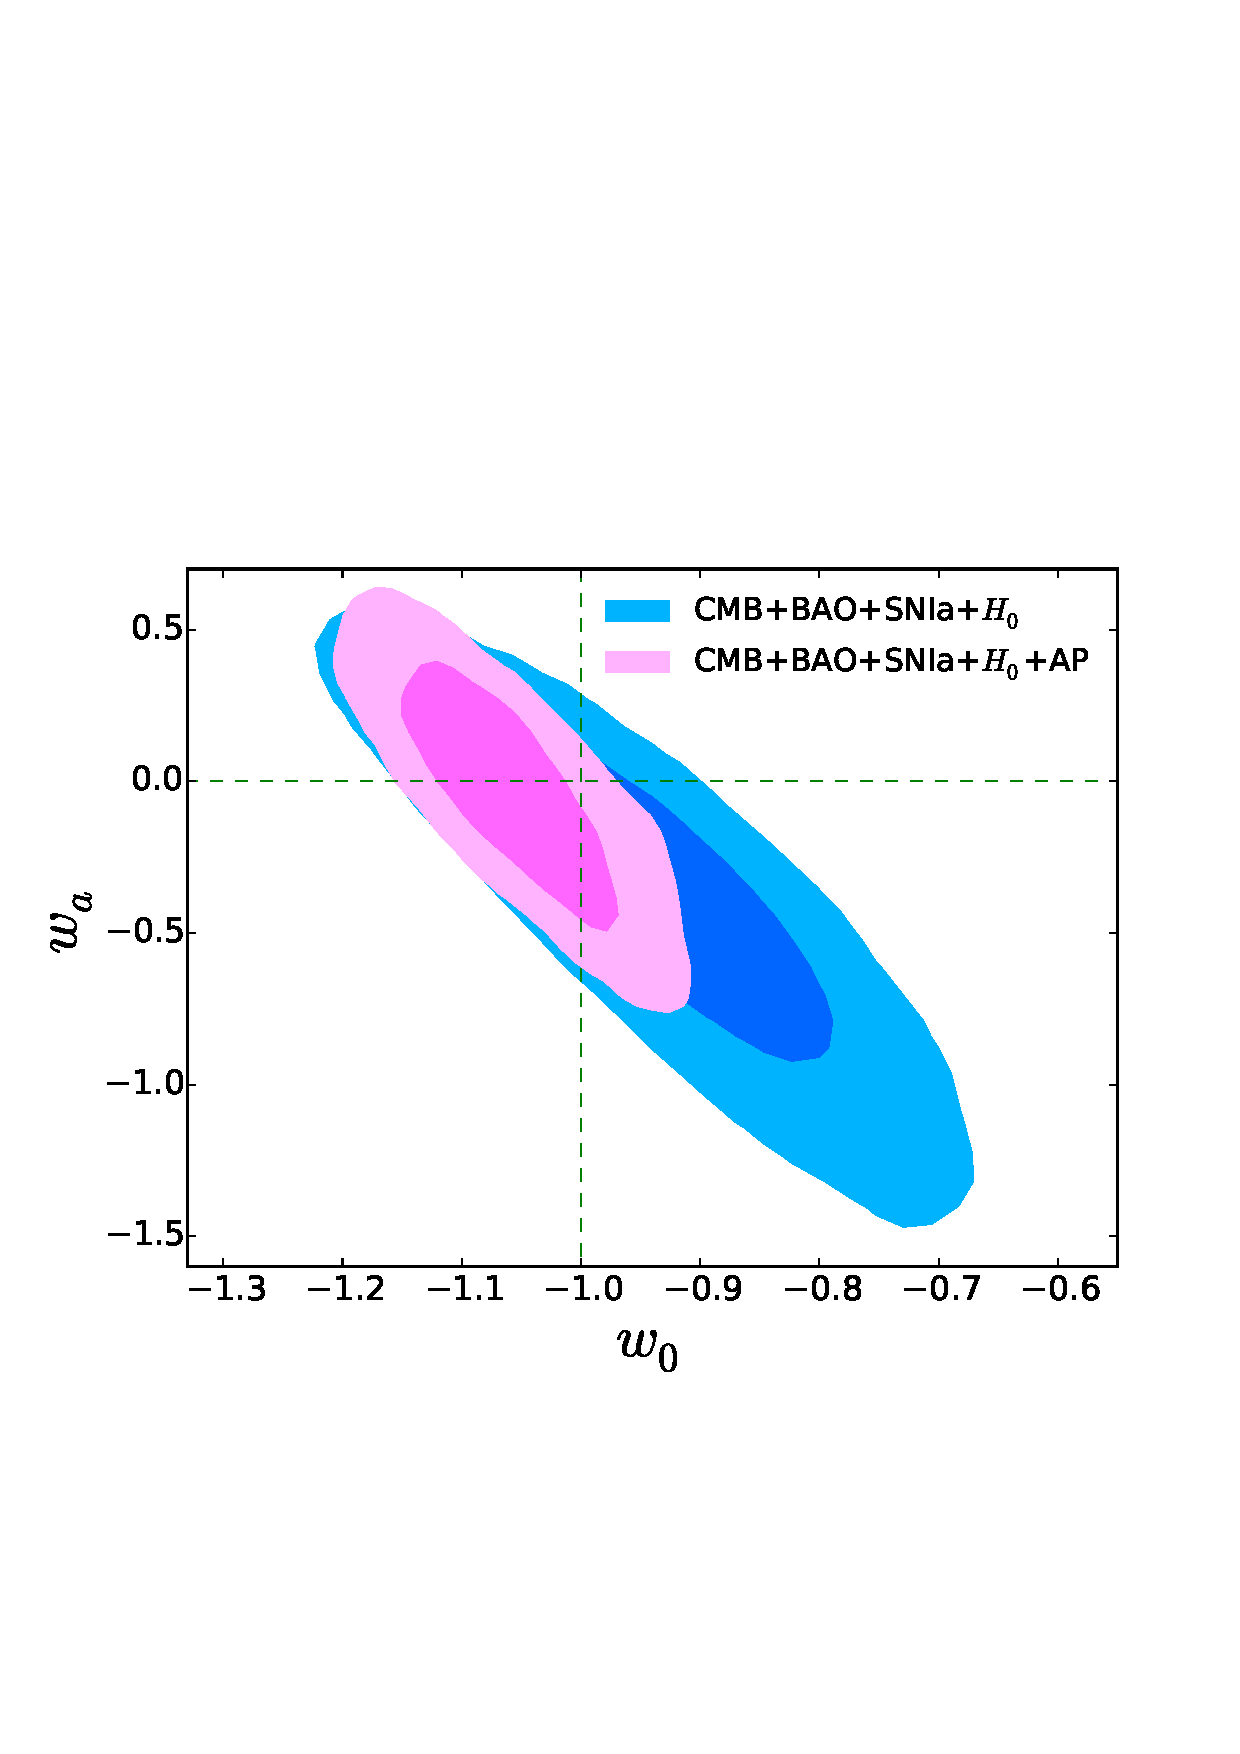
\includegraphics[height=8cm]{fig2b.pdf}
%   \includegraphics[height=8cm]{Tpcf--plot--Normed.eps}
%    \includegraphics[height=8cm]{smu.eps}
   }
   \caption{\label{fig_contest}
   Robustness test of the AP method. 
   For the ``default'' constraints (pink contours) are derived using six redshift bins, 
   $\mu_{\rm max}=0.97$, $n_{\mu}=15-20$, $s=6-40 \rm Mpc/h$,
   a fiducial cosmology $\Omega_m=0.26,\ w=-1.0$ for the measurement of 2pCF,
   systematic effects estimated from HR4 simulations, 
   and covariance estimated using 2,000 PATCHY mocks.
   When altering these options, the results remain robust (black contours).
   }
\end{figure}


\clearpage
\setcounter{page}{1}
\setcounter{figure}{0}
\setcounter{table}{0}

\begin{center}
{\textbf{ \Large \uppercase{Methods}} }
\end{center}

\noindent
%{\textbf{Target selection and data preparation.}}  
The spectroscopic galaxy sample of SDSS-III BOSS (Baryon Oscillation Spectroscopic Survey) has two primary catalogues:
%the LOWZ at $z\leq0.4$, and CMASS covering $0.4\leq z \leq 0.7$. %of galaxies.
the LOWZ sample, designed as an extension of the SDSS-I/II luminous red galaxy sample to $z\approx 0.4$ and fainter luminosities,
and the CMASS sample covers a higher redshift ($0.4\lesssim z \lesssim 0.7$),
targeted to be an approximately stellar mass limited sample of massive, luminous galaxies \cite{Reidetal:2016}.
In the clustering analysis we use 1,133,326 galaxies, split into six, non-overlapping redshift bins, 
$0.150<z_1<0.274<z_2<0.351<z_3<0.430<z_4<0.511<z_5<0.572<z_6<0.693$.
The number density of galaxies and the redshift binning scheme is plotted in the left panel of Fig.\ref{fig_TpCF}.

Following our previous methodology \citep{Li2016}, the information of small-scale anisotropic clustering is computed.
%\footnote{These correlations were computed using the public code \texttt{KSTAT} \citep{kstat}.} 
as $\xi_{\Delta s} (\mu) \equiv \int_{s_{\rm min}}^{s_{\rm max}} \xi (s,\mu)\ ds$, 
with $s_{\rm min}=6 h^{-1} {\rm Mpc},\ s_{\rm max}=40 h^{-1} {\rm Mpc}$.
We then normalise these {\em clustering shells} as 
$\hat\xi_{\Delta s}(\mu) \equiv \frac{\xi_{\Delta s}(\mu)}{\int_{0}^{\mu_{\rm max}}\xi_{\Delta s}(\mu)\ d\mu}$
to nullify the amplitude information of the clustering signal, 
which is not associated with the Alcock-Paczynski test and is mostly sensitive to the galaxy bias.

The right panel of Fig.\ref{fig_TpCF} shows the contour map of $\xi(s,\mu)$ measured in the six redshift bins.
The contour lines are not horizontal due to the effects of peculiar velocity,
and the RSD effect clearly manifest itself through the tilting of contour lines.
However, the shape of the tilted lines remain similar at different redshifts, a fact that enables us  to mitigate the RSD effect by focusing on the redshift dependence of the anisotropic clustering signal.
The ``correct'' cosmological model is selected by minimising the amount of redshift evolution of $\hat\xi_{\Delta s}$,
via a $\chi^2$ function of 
\begin{equation}
 \chi^2\equiv \sum_{i=2}^{6} \sum_{j_1=1}^{n_{\mu}} \sum_{j_2=1}^{n_{\mu}} {\bf p}(z_i,\mu_{j_1}) ({\bf Cov}_{i}^{-1})_{j_1,j_2}  {\bf p}(z_i,\mu_{j_2})
\end{equation}
where ${\bf p}(z_i,\mu_{j})$ is the redshift evolution of clustering with respect to the lowest redshift bin,
while subtracting systematic effects:
\begin{eqnarray}
 {\bf p}(z_i,\mu_{j}) \equiv\ & \left[\hat\xi_{\Delta s}(z_i,\mu_j)-\hat\xi_{\Delta s}(z_1,\mu_j)\right] \\ \nonumber
 &- \left[\hat\xi_{\Delta s}(z_i,\mu_j)-\hat\xi_{\Delta s}(z_1,\mu_j)\right]_{\rm sys}.
\end{eqnarray}
We use a number of $n_{\mu}$=20, 21, ... 25 bins for the value of $\hat\xi_{\Delta s}(\mu)$ at $0<\mu<\mu_{\rm max}$.
For the removal of fiber collision and the strong FoG effect near the LOS we take a cut $\mu_{\rm max} = 0.97$.

Systematics effects are estimated using mock catalogues derived from Horizon Run 4 (HR4) \cite{HR4},
an N-body simulation with box size $L={3150}$ $h^{-1}$Mpc, number of particles $6300^3$,   
initial redshift $z_{i}=100$, and WMAP5 cosmological parameters 
$(\Omega_{b},\Omega_{m},\Omega_\Lambda,h,\sigma_8,n_s)$  = (0.044, 0.26, 0.74, 0.72, 0.79, 0.96) \citep[]{komatsu 2011}. 
Mock galaxy samples are produced using a modified version of the one-to-one correspondence scheme \citep{hong2016}. 
The covariance matrix ${\bf Cov}$ is computed from the 2,000 sets of MultiDark PATCHY mock catalogues \citep{MDPATCHY}.
The statistical bias and scattering in the likelihood function (due to the finite number of mocks in covariance estimation) 
are corrected following \citet{Hartlap} and \citet{Percival2014}.

In \cite{Li2016} the likelihood contour of $\Omega_m-w$ was constructed by
measuring the 2PCF 3,375 times,
using 3D positions of BOSS galaxies computed in 71$\times$45 sets of cosmological parameters.
%with $0.06\leq \Omega_m\leq 0.41$, $-1.5 \leq w \leq -0.4$.
This procedure took 1 month using 500 cores of the KIAS {\texttt baekdu} cluster.
It would be too expensive to do such a computation on a 3D grid of $\Omega_m-w_0-w_a$,
so here we take an approach  of ``approximate 2PCF'', described as follows.

The number of pairs are only counted in a fiducial cosmology
-- which is taken as the $\Omega_m=0.26$ $\Lambda$CDM --
and ``translated'' to the measurements in a ``target'' cosmology using the relations, 
\begin{eqnarray}
 s_{\rm target} = s_{\rm fiducial} \sqrt{\alpha_{\parallel}^2 \mu_{\rm fiducial}+\alpha_{\bot}(1-\mu_{\rm fiducial}^2)}, \\
 \mu_{\rm target} = \mu_{\rm fiducial} \frac{\alpha_\parallel}
 {\sqrt{\alpha_{\parallel}^2 \mu_{\rm fiducial} +\alpha_{\bot}(1-\mu_{\rm fiducial}^2)}}
\end{eqnarray}
where $\alpha_{\bot}\equiv D_{A,\rm target}/D_{A,\rm fiducial}$,
$\alpha_{\parallel}\equiv H_{\rm fiducial}/H_{\rm target}$.
and values of $D_A$ and $H$ are computed in the effective redshifts of the six redshift bins.
In the fiducial cosmology
we measure $\xi(s,\mu)$ in an ultra high resolution of
$\Delta s = 0.2 {\rm Mpc/h}$, $\Delta \mu = 1/600$,
%Let us call this ``approximate 2pCF'' method.
%to obtain the accurate number counts 
and these small ``pixels'' are grouped to infer 
the number counts in other cosmologies, 
in large pixels of $\Delta s = 1 {\rm Mpc/h}$, $\Delta \mu = 1/120$.
%in the fiducial cosmology and group the bins in the target cosmology.
In the case when one small pixel belongs to more than one larger pixel (``edge effect'' ),
a correction is applied by computing the fraction of the overlapping area.
We found when using the approximate method the computed 
$\hat\xi_{\Delta s}(\mu)$ in a non-fiducial cosmology suffers from
an error of $\approx0.5\%$, which is 10 times smaller than 
the statistical noise in the 2pCF.

\noindent
{\textbf{Data availability.}} 
The codes computing the likelihood of the AP tests are available on GitHub,
\href{https://github.com/xiaodongli1986/APCPL.git}
{https://github.com/xiaodongli1986/APCPL.git}.
The codes computing the correlation functions are available via
\href{https://bitbucket.org/csabiu/kstat}
{https://bitbucket.org/csabiu/kstat}.
The MCMC chains for CPL are publicly available via the Planck Legacy Archive
\href{http://pla.esac.esa.int/pla/}
{http://pla.esac.esa.int/pla/}.
The COSMOMC software are publicly available and documented at
\href{http://cosmologist.info/cosmomc/}
{http://cosmologist.info/cosmomc/}.
The SDSS DR12 galaxy samples are publicly available and documented at
\href{https://data.sdss.org/sas/dr12/boss/lss/}
{https://data.sdss.org/sas/dr12/boss/lss/}.
The Horizun Run 4 simulation data is documented at
\href{http://sdss.kias.re.kr/astro/Horizon-Runs/Horizon-Run4.php}
{http://sdss.kias.re.kr/astro/Horizon-Runs/Horizon-Run4.php}.
To use the simulation data, contact directly Juhan Kim \href{kjhan@kias.re.kr}{kjhan@kias.re.kr}.


\begin{thebibliography}{10}
\setcounter{enumiv}{29}

\expandafter\ifx\csname url\endcsname\relax
  \def\url#1{\texttt{#1}}\fi
\expandafter\ifx\csname urlprefix\endcsname\relax\def\urlprefix{URL }\fi
\providecommand{\bibinfo}[2]{#2}
\providecommand{\eprint}[2][]{\url{#2}}

\bibitem[Ade et al. (2015)]{Planck2015}
Ade, P.A.R., Aghanim, N., \& Arnaud, M., et al. arXiv:1502.01589

\bibitem[Alam et al.(2016)]{Alam2016}
Alam, S., Ata, M., \& Bailey, S., et al. 2016,
submitted to MNRAS (arXiv:1607.03155)

%\bibitem[{{Alam} {et~al}\mbox{.}(2015{\natexlab{a}}){Alam}, {Albareti},
%  {Allende Prieto}, {Anders}, {Anderson}, {Anderton}, {Andrews}, {Armengaud},
%  {Aubourg}, {Bailey}, \& et~al.}]{dr12}
%{Alam} S., Albareti, F.D.,\& Allende Prieto, C., {et~al.}, 2015,  ApJS, 219, 12

\bibitem[Alcock \& Paczynski(1979)]{AP1979}
Alcock, C., \& Paczynski, B. 1979, Nature, 281, 358  

%\bibitem[Anderson et al.(2012)]{2012MNRAS.427.3435A} 
%Anderson, L., Aubourg, E., Bailey, S., et al.\ 2012, MNRAS, 427, 3435

\bibitem[Anderson et al.(2013)]{Anderson2013}
Anderson, L., Aubourg, \'E., \& Bailey, S. et al. 2014, MNRAS, 441, 24  
  
%\bibitem[Bassett et al.(2002)]{Bassett2002}
%Bassett, B.A., Kunz, M., Silk, J., \& Ungarelli, C. 2002, MNRAS, 336, 1217

\bibitem[Ballinger, Peacock \& Heavens 1996]{Ballinger1996}
Ballinger, W.E., Peacock, J.A., \& Heavens, A.F. 1996, MNRAS, 282, 877  

\bibitem[Betoule et al.(2014)]{JLA}
Betoule, M., Kessler, R., \& Guy, J., et al. 2014, A\&A, 568, 32


\bibitem[Beutler et al.(2011)]{6dFGS}
Beutler, F., Blake, C., \& Colless, M., et al. 2011, MNRAS, 416, 3017

\bibitem[Beutler et al.(2013)]{Beutler2013}
Beutler, F., Saito, S., \& Seo, H.-J., et al. 2013, MNRAS, 443, 1065

\bibitem[Beutler et al.(2016)]{Beutler2016}
Beutler, F., Seo, H.-J., \& Saito, S., et al. 2016,
arXiv:1607.03150

\bibitem[Blake et al.(2011)]{Blake2011}
Blake, C., Glazebrook, K., \& Davis, T. M., 2011, MNRAS, 418, 1725  

\bibitem[Blake et al.(2013)]{WiggleZtopoloy}
Blake, C., James, J.B., \& Poole, G.B. 2013, MNRAS, 437, 2488

\bibitem[Bolton et al.(2012)]{Bolton2012}
Bolton, A.S., Schlegel, \& D.J., Aubourg E., et al. 2012, AJ, 144, 144

\bibitem[Boylan-Kolchin et al.(2008)]{B08}
Boylan-Kolchin, M., Ma, C.-P., \& Quataert, E. 2008, MNRAS, 383, 93


%\bibitem[Bueno Belloso et al. (2012)]{BB2012}
%Bueno Belloso, A., Pettinari, G.W., Meures, N., \& Percival, W.J. 2012, Phys. Rev. D, 86, 023530

%\bibitem[Chevallier \& Polarski(2001)]{CP2001}
%Chevallier, M., Polarski, D. 2001, Int. J. Mod. Phys. D, 10, 213


%\bibitem[Choi et al.(2010)]{choi 2010}
%Choi, Y.-Y., Park, C., Kim, J., Gott, J.R., 
%Weinberg, D.H., Vogeley, M.S., \& Kim, S.S. 2010, ApJS, 190, 181

\bibitem[Christensen et al.(2001)]{Bayesian}
Christensen, N., Meyer, R., Knox, L., \& Luey, B. 2001, Class. Quant. Grav., 18, 2677

%\bibitem[Chuang et al.(2013)]{Chuang2013}
%Chuang, C.-H., Prada, F., Beutler, F., et al. 2013, arXiv:1312.4889  

\bibitem[Chuang \& Wang(2012)]{ChuangWang2012}
Chuang, C.-H., \& Wang, Y. 2012, MNRAS, 426, 226  


%\bibitem[Corasaniti \& Copeland(2003)]{Corasaniti2003}
%Corasaniti, P.S., Copeland, E.J. 2003, Phys. Rev. D, 67, 063521

%eBOSS: 
%http://arxiv.org/abs/1508.04473
\bibitem[Dawson et al.(2015)]{eBOSS}
Dawson, K.S., Kneib, J.P., \& Percival, W.J., et al. 2015, accepted AJ

\bibitem[Dawson et al.(2012)]{Dawson et al. 2012}
Dawson, K.S., Schlegel, D.J., \& Ahn, C.P., et al. 2012, AJ, 145, 10

\bibitem[Efstathiou (2014)]{E14H0}
Efstathiou, G. 2014, MNRAS, 440, 1138

\bibitem[Eisenstein et al.(2011)]{Eisenstein et al. 2011}
Eisenstein, D.J.,  Weinberg, D.H., \& Agolet, E., et al. 2011, AJ, 142, 72

\bibitem[Feldman, Kaiser \& Peacock (1994)]{1994ApJ...426...23F} 
Feldman, H.A., Kaiser, N., \& Peacock, J.A.\ 1994, ApJ, 426, 23 

\bibitem[Fukugita et al. (1996)]{Fukugita1996}
Fukugita, M., Ichikawa, T., \& Gunn, J.E., et al. 1996, AJ, 111, 1748
%Publication:	
%Astronomical Journal v.111, p.1748 

%\bibitem[Gingold \& Monaghan(1977)]{GM1977}
%Gingold, R.A., \& Monaghan, J.J. 1977, MNRAS, 181, 375  

%\bibitem[Gott et al.(2009)]{gott 2009}
%Gott, J.R., Choi, Y.-Y., Park, C., \& Kim, J. 2009, ApJ, 695, L45  

%\bibitem[Gott et al.(2008)]{gott 2008}
%Gott, J.R., Hambrick, D.C., Vogeley, M.S., Kim, J., Park, C., Choi, Y.-Y.,
%Cen, R., Ostriker, J.P., \& Nagamine, K. 2008, ApJ, 675, 16  


\bibitem[Gunn et al. (1998)]{Gunn1998}	
Gunn, J.E., Carr, M., \& Rockosi, C. et al. 1998, AJ, 116, 3040

\bibitem[Gunn et al.(2006)]{Gunn et al. 2006}
Gunn, J.E., Siegmund, W.A., \& Mannery, E.J., et al. 2006, AJ, 131, 2332

\bibitem[Guzzo et al.(2008)]{Guzzo2008}
Guzzo, L., Pierleoni, M., \& Meneux, B., et al. 2008, Nature, 451, 541

\bibitem[Hartlap et al.(2006)]{Hartlap}
Hartlap J., Simon P. \& Schneider P. [astro-ph/0608064].


\bibitem[Hong et al.(2016)]{hong2016}
Hong, S.E., Park, C.,\&  Kim, J. 2016, ApJ, 823, 103

\bibitem[Jackson (1972)]{FOG}
Jackson, J., 1972, MNRAS, 156, 1

\bibitem[Jennings et al.(2011)]{Jennings2011}
Jennings, E., Baugh, C.M., \& Pascoli, S. 2011, MNRAS, 420, 1079  

%\bibitem[Jeong et al.(2014)]{Jeong2014}
%Jeong, D., Dai, L., Kamionkowski, M., \& Szalay, A.S. 2014, arXiv:1408.4648

\bibitem[Jiang et al.(2008)]{jiang2008}
Jiang, C.Y., Jing, Y. P., \& Faltenbacher, A., et al. 2008, ApJ, 675, 1095

\bibitem[Kaiser (1987)]{Kaiser1987}
Kaiser, N. 1987, MNRAS, 227, 1


\bibitem[Kim \& Park(2006)]{kim and park 2006}
Kim, J., \& Park, C. 2006, ApJ, 639, 600  

\bibitem[Kim et al.(2009)]{2009ApJ...701.1547K} 
Kim, J., Park, C., Gott, J.R., III, \& Dubinski, J.\ 2009, ApJ, 701, 1547 

\bibitem[Kim et al.(2015)]{hr4}
Kim, J., Park, C., L'Huillier, B., \& Hong, S. E. 2015, JKAS, 48, 213

\bibitem[Kim et al.(2011)]{horizonrun}
Kim, J., Park, C., Rossi, G., Lee, S.M., \& Gott, J.R. 2011, JKAS, 44, 217  

\bibitem[Kitaura et al.(2015)]{MDPATCHY}
Kitaura, F.S., Rodriguez-Torres, S., Chuang, C.-H., et al. arXiv:1509.06400

\bibitem[Komatsu et al.(2011)]{komatsu 2011}
Komatsu, E., Smith, K. M., \& Dunkley, J., et al. 2011, ApJS, 192, 18  

\bibitem[Lacey \& Cole(1993)]{LC93}
Lacey, C., \& Cole, S. 1993, MNRAS, 262, 627


\bibitem[Landy \& Szalay(1993)]{1993ApJ...412...64L} 
Landy, S.D., \& Szalay, A.S.\ 1993, ApJ, 412, 64 

%EUCLID:
%http://arxiv.org/abs/1110.3193
\bibitem[Laureijs et al.(2011)]{EUCLID}
Laureijs, R., Amiaux, J., \& Arduini, S., et al. 2011, arXiv:1110.3193

\bibitem[Lavaux \& Wandelt(2012)]{LavausWandelt1995}
Lavaux, G., \& Wandelt, B.D. 2012, ApJ, 754, 109  

%\bibitem[Levi et al.(2013)]{2013arXiv1308.0847L} 
%Levi, M., Bebek, C., Beers, T., et al.\ 2013, arXiv:1308.0847 

\bibitem[Lewis \& Bridle (2002)]{LB2002}
Lewis, A., \& Bridle, S. 2002, Phys. Rev. D, 66, 103511

\bibitem[L'Huillier et al.(2014)]{2014NewA...30...79L} 
L'Huillier, B., Park, C., \& Kim, J.\ 2014, New Astronomy, 30, 79 

\bibitem[Li et al.(2011)]{Li2011}
Li, M., Li, X.-D., Wang, S., \& Wang, Y. 2011, Commun. Theor. Phys., 56, 525

\bibitem[Li et al.(2014)]{Li2014}
Li, X.-D., Park, C., Forero-Romero, J., \& Kim, J. 2014, ApJ, 796, 137

\bibitem[Li et al.(2015)]{Li2015}
Li, X.-D., Park, C., Sabiu, C.G., \& Kim, J. 2015, MNRAS, 450, 807 

\bibitem[Li et al.(2016)]{Li2016}
Li, X.-D., Park, C., \& Sabiu, C.G., et al. 2016, ApJ, 832, 103

%\bibitem[Linder(2003)]{Linder2003}
%Linder, E.V. 2003, Phys. Rev. Lett., 90, 091301

\bibitem[Linder et al.(2014)]{Linder2013}
Linder, E.V., Minji, O., Okumura, T., Sabiu, C.G., \& Song, Y.-S. 2014, Phys. Rev. D, 89, 063525  

\bibitem[L{\'o}pez-Corredoira(2014)]{2014ApJ...781...96L} 
L{\'o}pez-Corredoira, M.\ 2014, ApJ, 781, 96 

\bibitem[Mao et al. (2016)]{Qingqing2016}
Mao, Q., Berlind, A.A., Scherrer, R.J., et al. 2016, submitted to ApJ

\bibitem[Marinoni \& Buzzi(2010)]{Marinoni2010}
Marinoni, C., \& Buzzi, A. 2010, Nature, 468, 539  

\bibitem[Matsubara \& Suto(1996)]{Matsubara1996}
Matsubara T., \& Suto, Y. 1996, ApJ, 470, L1  

\bibitem[McCavana et al.(2012)]{M12}
McCavana, T., Micic, M., Lewis, G. F., et al. 2012, MNRAS, 424, 361


\bibitem[Morandi \& Sun (2016)]{MS2016}
Morandi, A., \& Sun, M. arXiv:1601.03741


\bibitem[Outram et al.(2004)]{Outram2004}
Outram, P.J., Shanks, T., Boyle, B.J., Croom, S.M., Hoyle, F., Loaring, N.S., 
Miller, L., \& Smith, R.J. 2004, MNRAS, 348, 745  

%\bibitem[Parejko et al.(2013)]{Parejko2013}
%Parejko, J. K., Sunayama, T., Padmanabhan, N., et al. 2013, MNRAS, 429, 98  

\bibitem[Parejko et al.(2013)]{Parejko2013}
Parejko J.K., et al., 2013, MNRAS, 429, 98

\bibitem[Parihar et al. (2014)]{CMASSLSS2014}
Parihar, P., Vogeley, M.S., \& Gott, J.R., et al. 2014, ApJ, 796, 86

\bibitem[Park et al.(2005)]{park 2005}
Park, C., Kim, J., \& Gott, J.R. 2005, ApJ, 633, 1  

\bibitem[Park \& Kim(2010)]{topology}
Park, C., \& Kim, Y.-R. 2010, ApJL, 715, L185  

\bibitem[Park et al. (2012)]{Park2012}
Park, C., Choi, Y.-Y., Kim, J., Gott, J.R., Kim, S.S., \&
Kim, K.-S. 2012, ApJ, 759, 7

\bibitem[Park et al. (2015)]{Park2015}
Park, C., Song, H., Einasto, M., Lietzen, H., \&
Heinamaki, P. 2015, JKAS, 48, 75

\bibitem[Peebles \& Ratra(2003)]{PR2003}
Peebles, P.J.E., \& Ratra, B. 2003, Reviews of Modern Physics, 75, 559

\bibitem[Percival et al.(2014)]{Percival2014}
Percival, W.J., Ross, A.J., \& S\'{a}nchez, A.G., et al. 2014, MNRAS, 439, 2531

\bibitem[Perlmutter et al.(1999)]{Perl1999}
Perlmutter, S., Aldering, G., \& Goldhaber, G., et al. 1999, ApJ, 517, 565  

\bibitem[Press \& Shechter(1974)]{PS1974}
Press, W.H., \& Schechter, P.L. 1974, ApJ, 187, 425



\bibitem[Reid et al.(2012)]{Reid2012}
Reid, B., Samushia, L., \& White, M., et al. 2012, MNRAS, 426, 2719  

\bibitem[Reid et al.(2016)]{Reidetal:2016}
Reid, B., Ho, S., \& Padmanabhan, N., et al.  2016, MNRAS, 455, 1553

\bibitem[Riess et al.(1998)]{Riess1998}
Riess, A.G., Filippenko, A.V., \& Challis, P., et al. 1998, AJ, 116, 1009  

\bibitem[Riess et al.(2011)]{Riess2011}
Riess, A.G., Macri, L., \& Casertano, S., et al. 2011, ApJ, 730, 119
%A 3\% Solution: Determination of the Hubble Constant with the Hubble Space Telescope and Wide Field Camera

\bibitem[Ross et al.(2012)]{2012MNRAS.424..564R} 
Ross, A.J., Percival, W.J., \& S{\'a}nchez, A.G. et al.\ 2012, MNRAS, 424, 564 

\bibitem[Ross et al.(2015)]{MGS}
Ross, A.J., Samushia, L., \& Howlett, C., et al. 2015, MNRAS, 449, 835

\bibitem[Ryden(1995)]{Ryden1995}
Ryden, B.S. 1995, ApJ, 452, 25  

%\bibitem[Samushia et al.(2014)]{Samushia2014}
%Samushia, L., Reid, B. A., White, M., et al. 2014, MNRAS, 439, 3504  

%\bibitem[Sanchez et al.(2013)]{Sanchez2013}
%Sanchez, A. G., Kazin, E. A., Beutler, F., et al. 2013, MNRAS, 433, 1202  

%\bibitem[Sutter et al.(2014)]{Sutter2014}
%Sutter, P.M., Pisani, A., Wandelt, B.D., \& Weinberg, D.H. 2014, MNRAS, 443, 2983


\bibitem[Sanchez et al.(2016)]{Sanchez2016}
Sanchez, A. G., Scoccimarro, R., \& Crocce, M., et al.
arXiv:1607.03147

\bibitem[Schlafly et al.(2010)]{Schlafly2010}
Schlafly E.F., Finkbeiner D.P., Schlegel D.J., et al. 2010, ApJ, 725, 1175

\bibitem[Schlafly \& Finkbeiner(2011)]{SF2011}
Schlafly E.F., \& Finkbeiner D.P. 2011, ApJ, 737, 103


%DESI:
%http://arxiv.org/abs/1106.1706
\bibitem[Schlegel et al.(2011)]{DESI}
Schlegel, D., Abdalla, F., \& Abraham, T., et al. 2011, arXiv:1106.1706

\bibitem[Smee et al.(2013)]{Smee2013}
Smee, S.A., Gunn, J.E., \& Uomoto, A., et al. 2013, AJ, 146, 32

\bibitem[Song et al.(2014)]{2014arXiv1407.2257S} 
Song, Y.S., Sabiu, C.G., 
Okumura, T., Oh, M., \& Linder, E.V.\ 2014, JCAP, 12, 005 

\bibitem[Speare et al. (2015)]{Speare2015}
Speare, R., Gott, J.R., Kim, J., \& Park, C.
2015, ApJ, 799, 176

%\bibitem[Tojeiro \& Percival(2011)]{Tojeiro2011}
%Tojeiro R., \& Percivial W.J. 2011, MNRAS, 417, 1114  

%\bibitem[Tojeiro et al.(2012)]{Tojeiro2012}
%Tojeiro, R., Percival, W. J., Wake, D. A., et al. 2012, MNRAS, 424, 136 

\bibitem[Viana \& Liddle(1996)]{VL1996}
Viana, P.T.P., \& Liddle, A.R. 1996, MNRAS, 281, 323

\bibitem[Villalobos et al.(2013)]{V13}
Villalobos, \'{A}., ́De Lucia, G., Weinmann, S.M., Borgani, S., \& Murante, G. 2013, MNRAS, 433, L49


\bibitem[Weinberg (1989)]{SW1989}
Weinberg, S. 1989, Reviews of Modern Physics, 61, 1

\bibitem[White (2011)]{White2011}
White M., et al. 2011, ApJ, 728, 126

\bibitem[Yoo \& Watanabe(2012)]{2012IJMPD..2130002Y} Yoo, J., \& Watanabe, Y.\ 2012, International Journal of Modern Physics D, 21, 1230002 

\bibitem[York et al.(2000)]{York et al. 2000}
York, D.G., Adelman, J., \& Anderson, J.E., et al. 2000, AJ, 120, 1579

\bibitem[Zehavi et al.(2011)]{zehavi2011}
Zehavi, I., Zheng, Z., \& Weinberg, D.H., et al. 2011, ApJ, 736, 59

\end{thebibliography}

%\clearpage
%\input{supplementaryinformation.tex}

\end{document}

